\chapter{Arquitectura y diseño}
\label{chap:arquitectura}


\section{Arquitectura general del sistema}
\label{sec:arquitectura}

El proyecto cuenta con cuatro nodos diferenciados, atendiendo cada uno a un subconjunto de los requisitos totales del proyecto agrupados por funcionalidades:

\begin{itemize}
    \item El modulo de captura y detección de posición
    \item El modulo de control de velocidad
    \item El modulo de actuación sobre el hardware
    \item El modulo de visualización
\end{itemize}

Esto permite el aislamiento del proyecto en sistemas independientes que se interconectan, enviando y recibiendo la información necesaria para su correcto funcionamiento através de la red, no pueden compartir un estado de memoria.

El funcionamiento del proyecto se lleva a cabo mediante la ejecución de un conjunto de nodos ROS~2 distribuidos en varias máquinas, que realizan la comunicación entre todos los nodos mediante la publicación y suscripción a \emph{topics} de ROS~2 y de una aplicación ejecutada en un Arduino cuyo hardware está conectado a la pista del Scalextric (ver figura~\ref{fig:arquitectura-general}). 

El \textbf{Modulo de captura y detección} está formado por un nodo cámara por cada cámara que observa el circuito, desplegado dentro de un contenedor Docker sobre la máquina a la que está conectada físicamente. Cada uno de estos nodos captura los fotogramas de su cámara, detecta en ellos los coches presentes en su porción visible del circuito y publica la posición de cada uno de ellos. 

El \textbf{Modulo de control del rail} se compone de un nodo controlador por cada raíl del circuito que, suscrito a las posiciones publicadas para su rail por cada uno de los nodos cámara, reconstruye la trayectoria del coche asignado a su carril y además utilizando las posiciones que recibe aplica un algoritmo cuyo objetivo es obtener el mejor valor del PWM para cada instante con el propósito de reducir al máximo el tiempo por vuelta. Cada uno de los nodos publica el valor de PWM correspondiente a su caril, para vez que el nodo camara procesa un fotograma y publica la ubicación del coche.

El \textbf{Modulo actuación} centraliza en un único nodo la comunicación con el Arduino los valores de PWM publicados por todos los controladores, trasladándoselos a la aplicación Arduino, que aplica la tensión correspondiente a cada carril de la pista a través de un controlador L293D. La comunicación entre este nodo y el Arduino se lleva a cabo mediante un puerto serie USB conectado al Arduino.

El \textbf{Modulo de visualización y logging} se compone de un nodo de captura que se suscribe a la información de telemetría publicada por el resto del sistema y la almacena dentro de un bag de ROS2. Por otro lado existe un nodo de visualización que permite al usuario supervisar el estado de la carrera en directo y luego en diferido acceder a un analisis de las estadisticas, apartir del bag que genera el otro nodo. 

\begin{figure}[tbp]
    \centering
    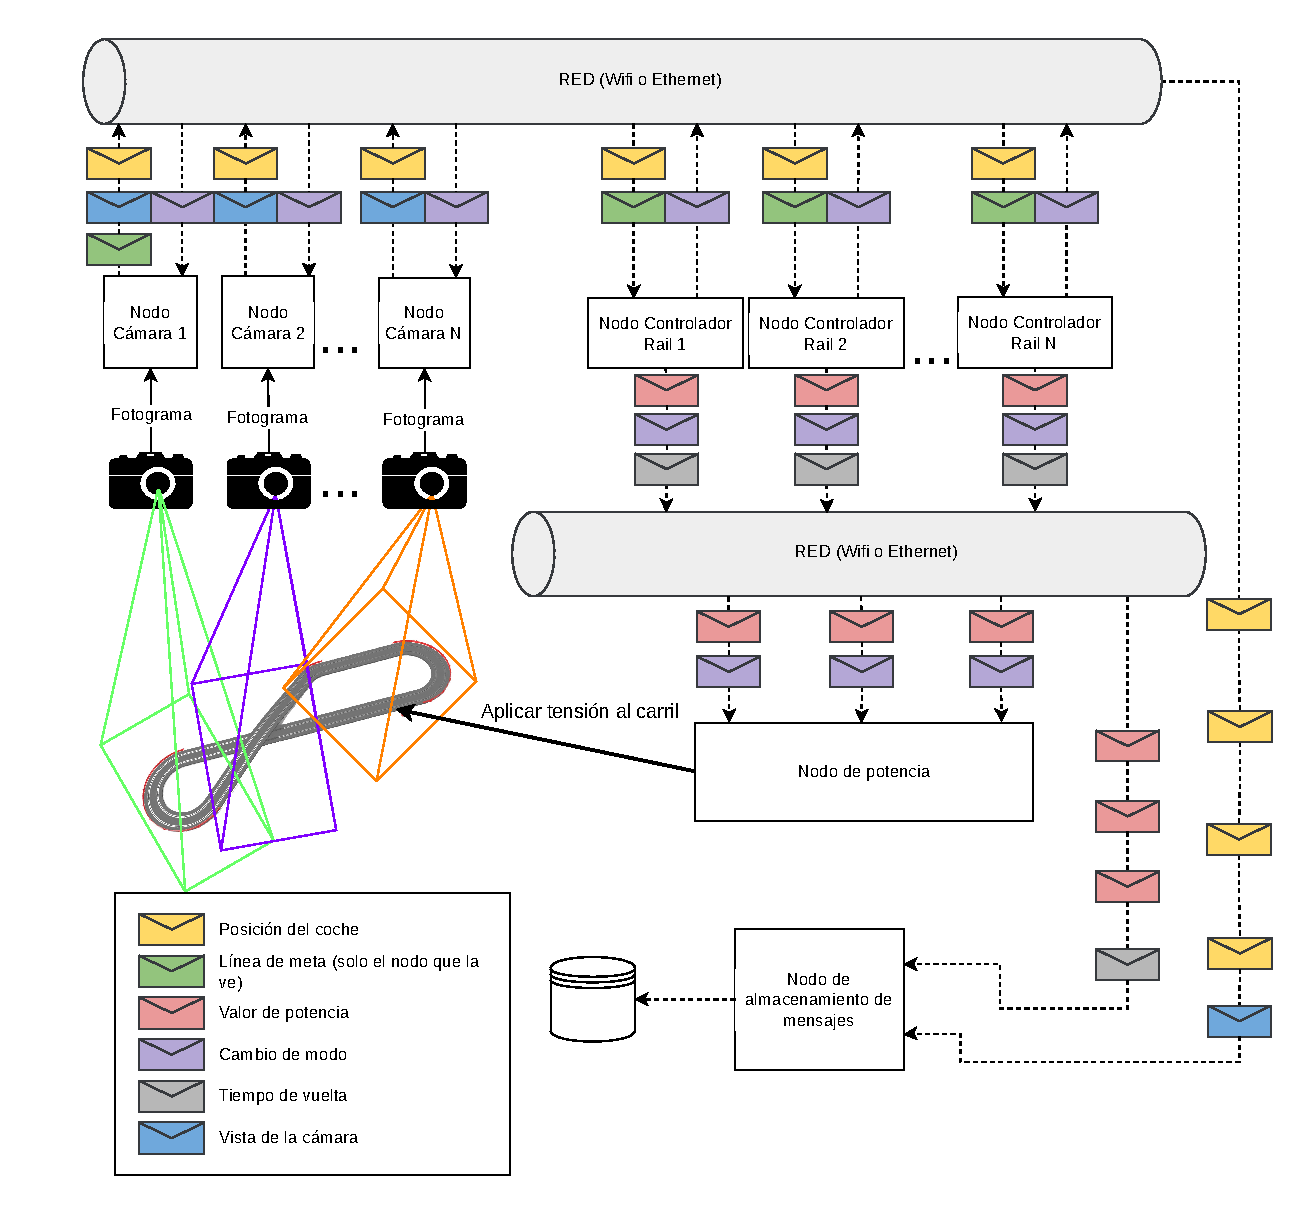
\includegraphics[width=1\textwidth]{imaxes/ARQUITECTURA/Arquitectura_General_Sistema.pdf}
    \caption{Arquitectura general del sistema pensado para el control distribuido de coches tipo scalextric con visión por computado}
    \label{fig:arquitectura-general}
\end{figure}

\section{Modelo de datos}
\label{sec:modelo_datos}

\section{Modos funcionamiento}
\label{sec:modos_funcionamiento}

\section{Algoritmo}
\label{sec:algoritmo}

\section{Intercambio de información(Qos)}
\label{sec:intercambio_informacion}

\section{Modelo concurrente}
\label{concurrencia}
